% M* scheme stencil
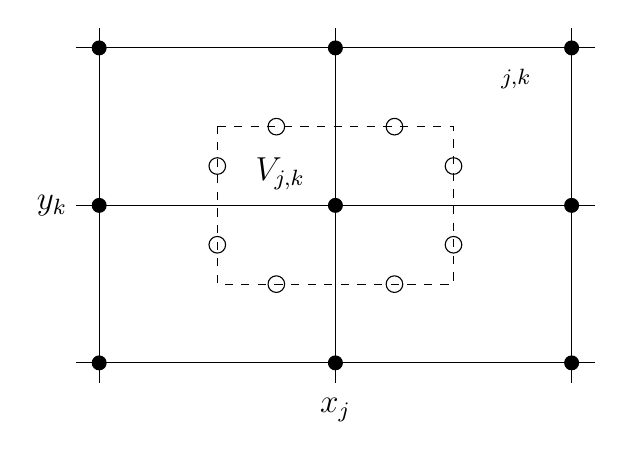
\begin{tikzpicture}[scale=1.0]
  % strong grid around elements beyond 0 and 6 in x and 0 and 4 in y
  \draw (-0.3,0) -- (6.3,0);
  \draw (-0.3,2) -- (6.3,2);
  \draw (-0.3,4) -- (6.3,4);
  \draw (0,-0.25) -- (0,4.25);
  \draw (3,-0.25) -- (3,4.25);
  \draw (6,-0.25) -- (6,4.25);

  % nodes
  \filldraw (0,0) circle (2.5pt);  \filldraw (3,0) circle (2.5pt);  \filldraw (6,0) circle (2.5pt);
  \filldraw (0,2) circle (2.5pt);  \filldraw (3,2) circle (2.5pt);  \filldraw (6,2) circle (2.5pt);
  \filldraw (0,4) circle (2.5pt);  \filldraw (3,4) circle (2.5pt);  \filldraw (6,4) circle (2.5pt);

  % outline control volume
  \draw[dashed] (1.5,3) -- (4.5,3) -- (4.5,1) -- (1.5,1) -- cycle;

  % mark quadrature points
  \draw (4.5,2.5) circle (3.0pt);
  \draw (3.75,3)  circle (3.0pt);
  \draw (2.25,3)  circle (3.0pt);
  \draw (1.5,2.5) circle (3.0pt);
  \draw (1.5,1.5) circle (3.0pt);
  \draw (2.25,1)  circle (3.0pt);
  \draw (3.75,1)  circle (3.0pt);
  \draw (4.5,1.5) circle (3.0pt);

  % label elements and control volume
  \draw (2.3,2.4) node {\large $V_{j,k}$};
  \draw (5.3,3.6) node {\large $\square_{j,k}$};

  % label center point
  \draw (3,-0.6) node {\large $x_j$};
  \draw (-0.6,2) node {\large $y_k$};
\end{tikzpicture}

